\documentclass[tikz]{standalone}
% \usepackage{tikz} % already loaded by the documentclass


\begin{document}
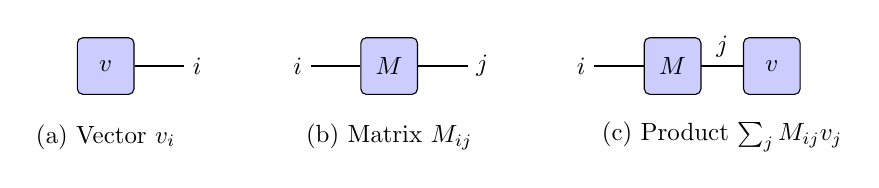
\begin{tikzpicture}[
    scale=0.9, every node/.style={scale=0.9},
    tensor/.style={draw,fill=blue!20,rounded corners=2pt,minimum size=8mm},
  ]
  % Vector
  \node[tensor] (v) at (0,0) {$v$};
  \draw[-] (v.east) -- ++(0.7,0) node[right] {$i$};
  \node at (0, -1) {(a) Vector $v_i$};

  % Matrix
  \node[tensor] (M) at (4,0) {$M$};
  \draw[-] (M.west) -- ++(-0.7,0) node[left] {$i$};
  \draw[-] (M.east) -- ++(0.7,0) node[right] {$j$};
  \node at (4, -1) {(b) Matrix $M_{ij}$};

  % Matrix-Vector Product
  \node[tensor] (M2) at (8,0) {$M$};
  \node[tensor] (v2) at (9.4,0) {$v$};
  \draw[-] (M2.west) -- ++(-0.7,0) node[left] {$i$};
  \draw[-] (M2.east) -- (v2.west) node[midway,above] {$j$};
  \node at (8.7, -1) {(c) Product $\sum_j M_{ij} v_j$};
\end{tikzpicture}
\end{document}
      